%%%%%%%%%%%%%%%%%%%
% MOTIVATION
%%%%%%%%%%%%%%%%%%%
\def\title{KBP: Directly find facts in text}
\begin{frame}{\title}
\begin{center}
  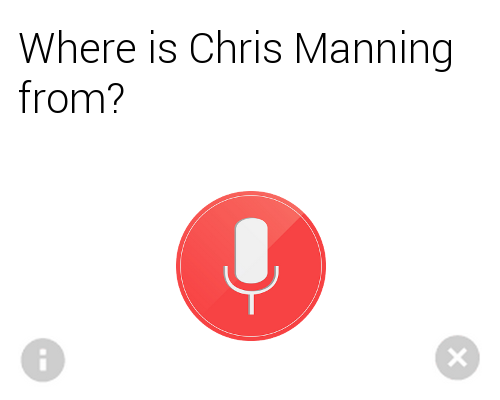
\includegraphics[width=7cm]{../img/google-chris-manning-origin.png}
\end{center}
\end{frame}

\begin{frame}[noframenumbering]{\title}
\vspace{-1cm}
\begin{center}
  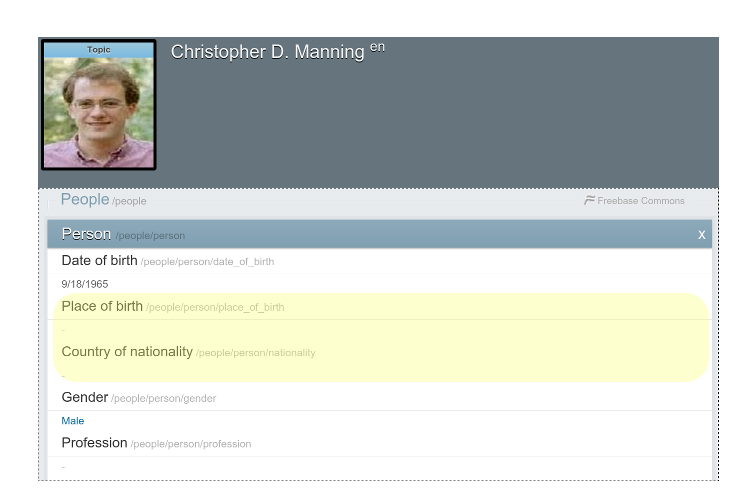
\includegraphics[width=10.5cm]{../img/chris-freebase.png}
\end{center}
\end{frame}

\begin{frame}[noframenumbering]{\title}
\begin{center}
  \begin{tabular}{l}
  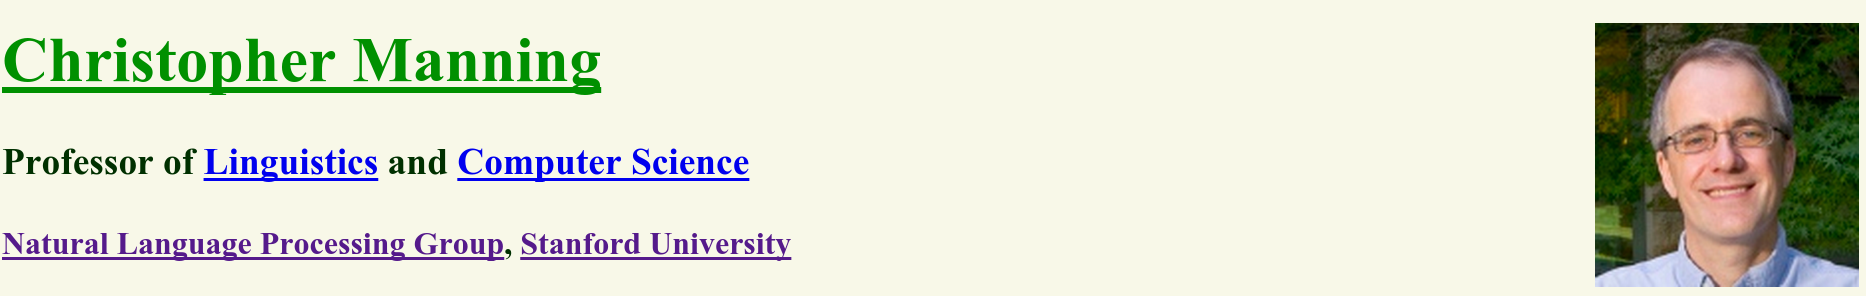
\includegraphics[width=12cm]{../img/chris-website-header.png} \\
  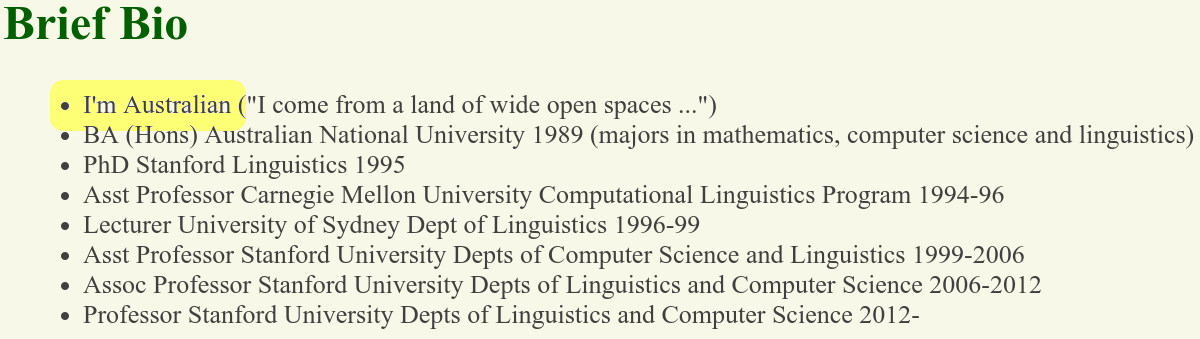
\includegraphics[width=9cm]{../img/chris-bio.png}
  \end{tabular}
\end{center}
\end{frame}

\begin{frame}[noframenumbering]{\title}
\begin{center}
  \fbox{
\includegraphics[width=7cm]{../img/google-chris-manning-origin-answer.png}}
\end{center}
\end{frame}

%%%%%%%%%%%%%%%%%%%%
%% INTRO
%%%%%%%%%%%%%%%%%%%%
%\begin{frame}{We're filling a fixed relation schema}
%\begin{center}
%\begin{tabular}{cccc}
%  \begin{tabular}{c}
%    \h{Unstructured Text} \\
%    \\
%    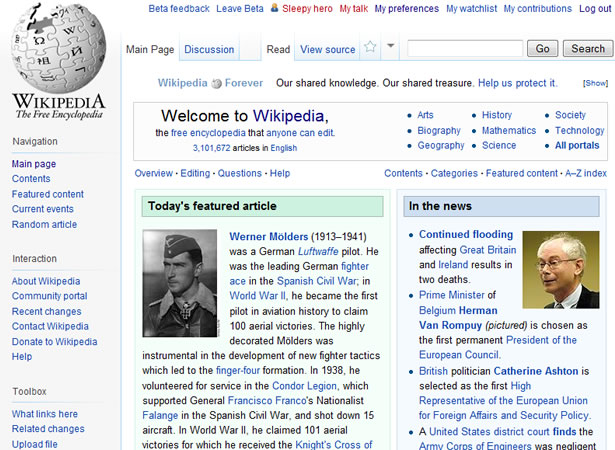
\includegraphics[width=2cm]{../img/wiki.jpg} \\
%    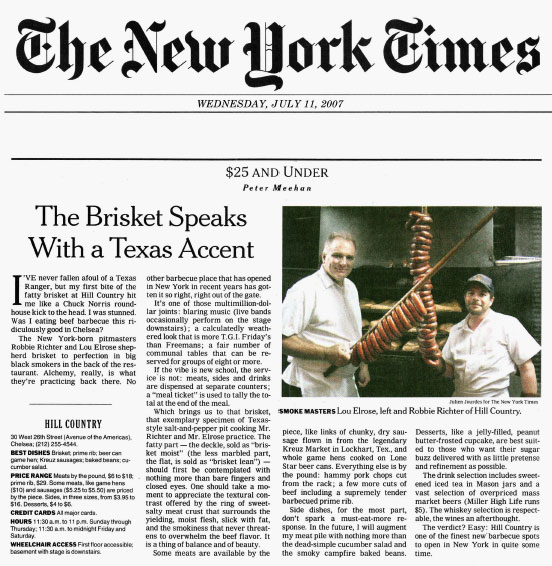
\includegraphics[width=2cm]{../img/nyt.jpg} \\
%    
\includegraphics[width=2cm]{../img/blog.jpg}
%  \end{tabular} &
%
%  \Huge{$\Rightarrow$} &
%  
%  \begin{tabular}{c}
%  \h{Structured Knowledge Base} \\
%  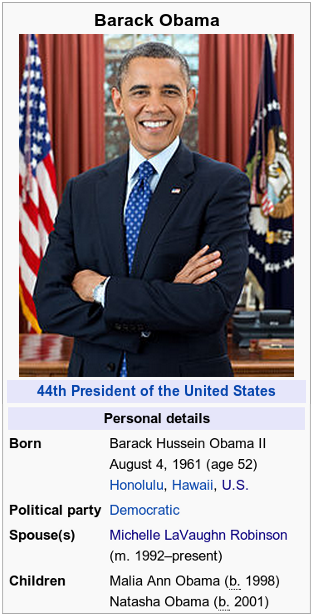
\includegraphics[width=2.75cm]{../img/obama-infobox.png}
%  \end{tabular}
%\end{tabular}
%\end{center}
%\end{frame}


%%%%%%%%%%%%%%%%%%%
% RELATION EXTRACTION
%%%%%%%%%%%%%%%%%%%
\begin{frame}{Active Learning for Relation Extraction}
  \hh{Input}:  Sentences containing (\subj{entity}, \obj{slot value}). \\
  \hh{Output}: \rel{Relation} between \subj{entity} and \obj{slot value}.
  \pause
  \vspace{1cm}

  \hh{Consider two approaches:} \begin{itemize}
    \item \h{Supervised:} Trivial as a supervised classifier. \\
      Training data: \{(sentence, relation)\}. \\
      \textit{But}$\dots$ \pause this training data is expensive to produce.
    \pause
    \vspace{0.5cm}
  
    \item \h{Distantly Supervised:} Artificially produce ``supervised'' data. \\
      Training data: \{(\subj{entity}, relation, \obj{slot value})\}. \\
      \textit{But}$\dots$ \pause this training data is much more noisy.
  \end{itemize}
\end{frame}

%%%%%%%%%%%%%%%%%%%
% CONTRIBUTIONS
%%%%%%%%%%%%%%%%%%%
\begin{frame}{Active Learning: Combine Benefits of Both}
\begin{center}
  \hh{Adding carefully selected supervision improves
      distantly supervised relation extraction.}
\end{center}
\vspace{0.5cm}
\pause

\hh{Old problem:}  Supervision is expensive,
  but very useful. \\
\vspace{0.25cm}
\hh{Old solution:} Active learning! \\
\pause
\begin{itemize}
  \item Select a subset of sentences to annotate.
  \item Fix these labels during training.
%  \pause
%  \item Bonus: this creates a supervised training set.
%  \begin{itemize}
%    \item We initialize from a supervised classifier on this training set.
%  \end{itemize}
\end{itemize}

\end{frame}

%%%%%%%%%%%%%%%%%%%
% RESULTS: CRITERIA IMPORTANT (MIHAI)
%%%%%%%%%%%%%%%%%%%
\begin{frame}{State-of-the-art results}
\hh{Slot filling evaluation of Surdeanu et al. (2012).}
\begin{center}
  \includegraphics<1-1>[height=6cm]{../mihaiPRCurves/evaluateCriteriaSup_0}
  \includegraphics<2-2>[height=6cm]{../mihaiPRCurves/evaluateCriteriaSup_1}
%  \includegraphics<3-3>[height=6cm]{../mihaiPRCurves/evaluateCriteriaSup_2}
%  \includegraphics<4-4>[height=6cm]{../mihaiPRCurves/evaluateCriteriaSup_3}
  \includegraphics<3-3>[height=6cm]{../mihaiPRCurves/showNetImprovement_0}
  \includegraphics<4-4>[height=6cm]{../mihaiPRCurves/showNetImprovement_1}
\end{center}
\end{frame}

\begin{frame}[noframenumbering]{State-of-the-art results}
\hh{Slot filling evaluation of Surdeanu et al. (2012).}
\begin{center}
  \includegraphics<1-1>[height=6cm]{../mihaiPRCurves/compareToOthers}
\end{center}
\end{frame}

